\documentclass{amsart}

\usepackage{graphicx, fancyhdr, rotating, float} % see geometry.pdf on how to lay out the page. There's lots.
\usepackage[a4paper, margin=0.5in, includeheadfoot, headheight=2cm, footskip=2cm]{geometry}
\usepackage{booktabs}
\usepackage{multirow}


\usepackage{color}
\usepackage{xcolor}
\usepackage{listings}
\usepackage{numprint}
\npthousandsep{,}

\usepackage{caption}
\DeclareCaptionFont{white}{\color{white}}
\DeclareCaptionFormat{listing}{\colorbox{gray}{\parbox{\textwidth}{#1#2#3}}}
\captionsetup[lstlisting]{format=listing,labelfont=white,textfont=white}



% See the ``Article customise'' template for come common customisations
\providecommand{\e}[1]{\ensuremath{\times 10^{#1}}}
%\setlength{\headheight}{2cm}

\graphicspath{{./images/}} % Specify images directory


% Title and document details
\newcommand{\titleinfo}{$job.title} 
\title{\titleinfo}
\pagestyle{fancy}
\fancyhf{}
\lhead{}
\chead{
\includegraphics[height=2.5cm]{header.png}}
\renewcommand{\headrulewidth}{0pt}
\rhead{}
\rfoot{\thepage}
\lfoot{\titleinfo}
\author{$job.author}
\date{\today}

%%% BEGIN DOCUMENT
\begin{document}

% First page (title and toc)
\maketitle
\thispagestyle{fancy}
\tableofcontents


% General spacing for the document to use after the title and toc
\linespread{1.2} % A little more line spacing than usual
\setlength\parindent{0pt} % Removes indentation from paragraphs
\setlength{\parskip}{0.25cm} % Adds an extra bit of linespacing between paragraphs
\setlength{\belowbottomsep}{2ex} % Ensure a decent gap before the footer



\newpage
\section{General Information}
\begin{description}
\item[Project title] \titleinfo
\item[Name of collaborator] $job.collaborator
\item[Staff member] $job.author
\item[SEQINFO ticket] $job.jiraSeqinfoId
\item[MISO ticket] $job.misoId
\item[Date at job completion] \today
\end{description}


\section{Software Used}

This first pass assembly was built with RAMPART (Robust Automatic MultiPle Assembly Toolkit).  RAMPART is an TGAC project that chains a number of other tools together into a workflow.  The used for this job are specified in Table \ref{tab:software-used}.

\begin{table}[h]
\begin{tabular}{lll}
\toprule
Task & Tool & Version \\ \midrule
Quality Trimming & $tool.getQtName() & $tool.getQtVersion() \\
Contig Assembly & $tool.getMassName() & $tool.getMassVersion() \\
Scaffolding & $tool.getImpScfName() & $tool.getImpScfVersion() \\
Gap Closing & $tool.getImpDegapName() & $tool.getImpDegapVersion() \\
\bottomrule
\end{tabular}
\caption{Software used for this RAMPART job.}
\label{tab:software-used}
\end{table}


\pagebreak
\newpage
\section{Diagrammatic Representation of the Complete Workflow}

Figure \ref{fig:workflow} represents the general workflow applied to the raw reads produced from the sequencing device.  Initially multiple datasets are produced, then each of these is processed through an assembler using multiple k-mer values producing multiple assemblies.  These assemblies are analysed and the best assembly is selected to be enhanced using multiple iterations of SSPACE and GapCloser.  The resulting file has scaffolds under 1KB removed before a final screening process is applied.

\begin{figure}[H]
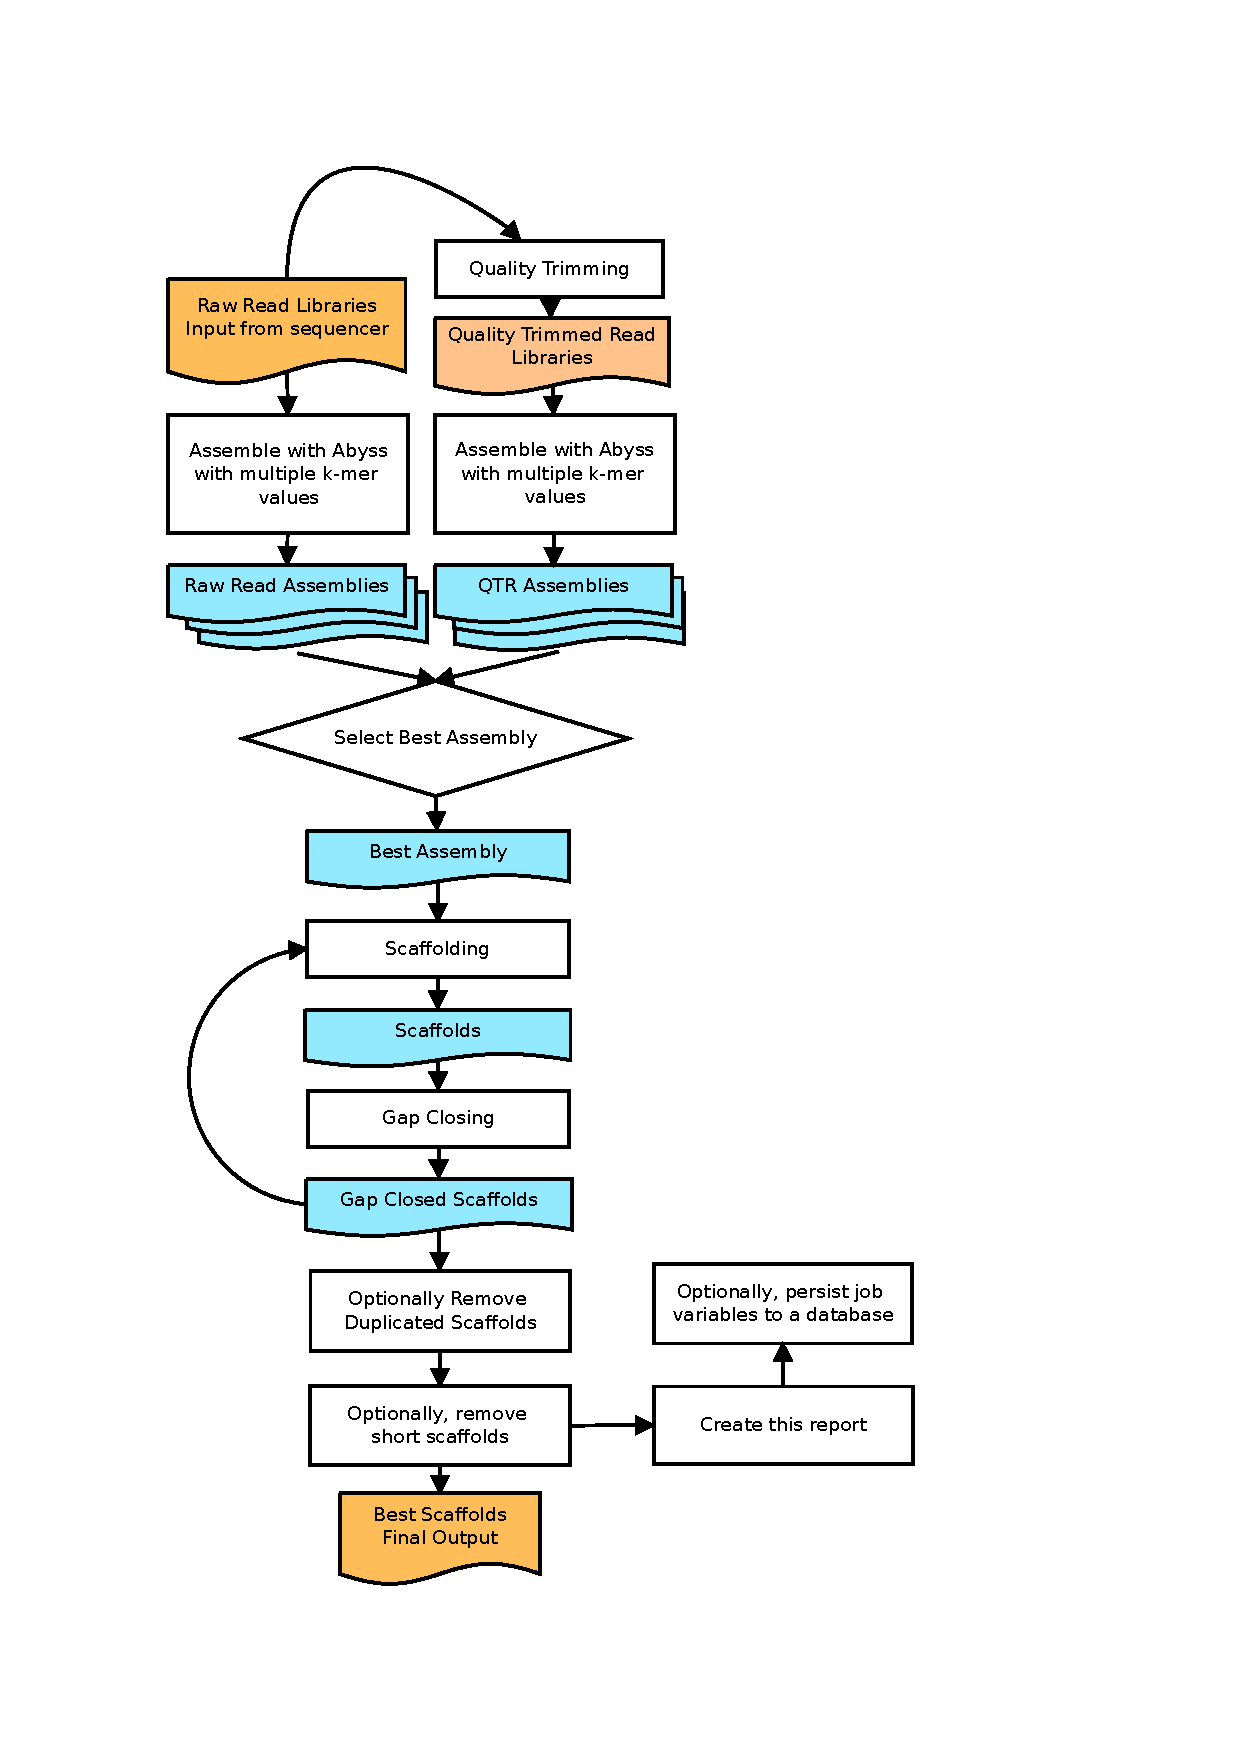
\includegraphics[width=13cm]{Workflow.pdf}
\caption{Typical First Pass Assembly Workflow}
\label{fig:workflow}
\end{figure}

\newpage
\section{Quality Trimming}

The job requested the raw sequenced libraries specified in Table \ref{tab:libraries}.  The reads in these libraries were analysed based on the sequence quality scores, and those sequences which dipped below a certain threshold were either trimmed or excluded.  $tool.qtName was used to do this.  This tool was configured so that the 3' ends of reads are trimmed where quality degrades beyond a threshold score of Q-$tool.qtThreshold.  Any trimmed reads must still exceed $tool.qtMinLen base pairs in length otherwise the whole read is discardedimages.  The dataset statistics before and after quality trimming are shown in Table \ref{tab:dataset-stats}.

\begin{table}[h]
\begin{tabular}{lrrll}
\toprule
Library Name & Maximum Read Length & Average Read Length & Usage & Orientation \\ \midrule
#foreach($lib in $job.libsRaw)
$lib.name & $lib.readLength & $lib.averageInsertSize & $lib.usage.toString() & $lib.seqOrientation \\
#end
\bottomrule
\end{tabular}
\caption{Libraries used for this RAMPART job.}
\label{tab:libraries}
\end{table}

\begin{table}[h]
\begin{tabular}{lllrrrr}
\toprule
Library & Dataset & File & Total Unpaired Reads & \%GC & Total Bases & Estimated Coverage  \\ \midrule
#foreach($lib in $job.libsRaw)
$lib.name & $lib.dataset & PE1 & \numprint{$lib.filePaired1.seqCount} & $lib.filePaired1.gCContent & \numprint{$lib.filePaired1.baseCount} & $0 \times$ \\ 
$lib.name & $lib.dataset & PE2 & \numprint{$lib.filePaired2.seqCount} & $lib.filePaired2.gCContent & \numprint{$lib.filePaired2.baseCount} & $0 \times$ \\
#if( $lib.seFile )
$lib.name & $lib.dataset & SE & \numprint{$lib.seFile.seqCount} & $lib.seFile.gCContent & \numprint{$lib.seFile.baseCount} & $ xxx \times$ \\
#end
#end
#foreach($lib in $job.libsQt)
$lib.name & $lib.dataset & PE1 & \numprint{$lib.filePaired1.seqCount} & $lib.filePaired1.gCContent & \numprint{$lib.filePaired1.baseCount} & $0 \times$ \\ 
$lib.name & $lib.dataset & PE2 & \numprint{$lib.filePaired2.seqCount} & $lib.filePaired2.gCContent & \numprint{$lib.filePaired2.baseCount} & $0 \times$ \\
#if( $lib.seFile )
$lib.name & $lib.dataset & SE & \numprint{$lib.seFile.seqCount} & $lib.seFile.gCContent & \numprint{$lib.seFile.baseCount} & $ xxx \times$ \\
#end
#end
\bottomrule
\end{tabular}
\caption{Basic Statistics for each library before and after quality trimming (Dataset `RAW' indicates before quality trimming and `QT' indicates after quality trimming.  #if($job.estGenomeSize) Estimated Coverage assumes even distribution of reads against a genome size of $job.estGenomeSizeMb.#end}
\label{tab:dataset-stats}
\end{table}



\newpage
\section{Multiple Contig Assemblies}

The datasets we assembled the reads by $tool.massName $tool.massVersion using a variety of k-mer lengths.  Various contig size metrics were gathered from each contig assembly in order to determine the optimal k-mer setting from which to build the final scaffolded assembly.  Graphs generated from some of the key size metrics across all k-mer values are shown in Table \ref{fig:contig_assembly_graphs}.

\begin{table}[H]
\begin{center}
\begin{tabular}{c|c|c}
\includegraphics[height=5cm]{Mass_NBC.pdf} & \includegraphics[height=5cm]{Mass_TB.pdf} & \includegraphics[height=5cm]{Mass_N.pdf}\\ \midrule 
\includegraphics[height=5cm]{Mass_AL.pdf} & \includegraphics[height=5cm]{Mass_ML.pdf} & \includegraphics[height=5cm]{Mass_N50.pdf} 
\end{tabular}
\end{center}
\caption{Plots showing various assembly size metrics against kmer value. Black lines represent the Raw Dataset.  Red lines the quality trimmed dataset. }
\label{fig:contig_assembly_graphs}
\end{table}

RAMPART normalises and weights contig assembly statistics in order to generate an overall assembly quality score.  The weightings related to each size metric are shown in Table \ref{tab:weightings}.  The overall contig assembly scores are shown in Table \ref{tab:contig_assembly_scores}.  The contig assembly that scores the maximum value has a k-mer value of $best_mass_asm.kmer and it was from the $best_mass_asm.dataset dataset.

\begin{table}
\begin{center}
\begin{tabular}{lr}
\toprule
Metric & Weighting \\ \midrule
#foreach($weighting in $weightings)
$weighting.name & $weighting.value \\
#end
\bottomrule
\end{tabular}
\end{center}
\caption{Weightings applied to each assembly size metric.}
\label{tab:weightings}
\end{table}

\begin{table}
\begin{center}
\begin{tabular}{llr}
\toprule
Kmer & Dataset & Score \\ \midrule
#foreach($score in $contigScores)
$score.kmer & $score.datset & $score.score \\
#end
\bottomrule
\end{tabular}
\end{center}
\caption{Overall contig assembly scores.}
\label{tab:contig_assembly_scores}
\end{table}




\newpage
\section{Assembly Enhancement}

The best contig assembly was then enhanced through a process of scaffolding and gap closing.  $tool.getImpScfName() $tool.getImpScfVersion() was used for scaffolding.  $tool.getImpDegapName() $tool.getImpDegapVersion() was used for the gap closing. #if($tool.getImpIterations() > 1) These two steps were repeated $tool.getImpIterations() times.#end  The results of this step are shown in the Figure \ref{fig:scaffold_assembly_graphs}.

#if($tool.impDedup)
After scaffolding and gap closing the scaffolds which describe subsets of other scaffolds are discarded.
#end

#if($tool.impClip)
Finally, scaffolds shorter than $tool.impClipMinLen were discarded from the final assembly.
#end

\begin{table}[H]
\begin{center}
\begin{tabular}{c|c|c}
\includegraphics[height=5cm]{Improver_NBC.pdf} & \includegraphics[height=5cm]{Improver_TB.pdf} & \includegraphics[height=5cm]{Improver_N.pdf}\\ \midrule 
\includegraphics[height=5cm]{Improver_AL.pdf} & \includegraphics[height=5cm]{Improver_ML.pdf} & \includegraphics[height=5cm]{Improver_N50.pdf} 
\end{tabular}
\end{center}
\caption{Plots showing various assembly size metrics against enhancement stage.}
\label{fig:scaffold_assembly_graphs}
\end{table}

The final assembly has $final_asm.nbContigs, and contains $final_asm.nbBases.  The average scaffold length is $final_asm.avgLen and the maximum scaffold length is $final_asm.maxLen.  Finally, the N50 score is $final_asm.n50.


\newpage
\section{Validation}

No validation on the final assembly is done at present.  In the future though we expect to be able to tell you about many more assembly quality metrics.


\newpage
\section{Accessing the Data}

The RAMPART job directory is located at:

\begin{lstlisting}[label=path:1]
$locations.getJobDir()
\end{lstlisting}

The original reads, as well as the quality trimmed reads can be found at the following location:

\begin{lstlisting}[label=path:1]
$locations.getReadsDir()
\end{lstlisting}

\emph{Note}: The quality trimmed read files referred to in this report can be identified with the *.qt.* tag.

The Abyss assemblies and statistics for each dataset can be found at the following location:

\begin{lstlisting}[label=path:1]
$locations.getMassDir()
\end{lstlisting}


The assemblies, statistics and other data for the assembly improvement stage can be found at the following location:

\begin{lstlisting}[label=path:1]
$locations.getImproverDir()
\end{lstlisting} 


The final assembly can be found at the following location:

\begin{lstlisting}[label=path:1]
$final_asm.getFilePath()
\end{lstlisting}


\end{document}

